\begin{frame}{Monte-Carlo photon reconstruction (2)}
Example of fits:
  \setlength{\unitlength}{1mm}
  \centering
  \scalebox{0.5}{
  \begin{picture}(225,120)
    \put(0,60){
      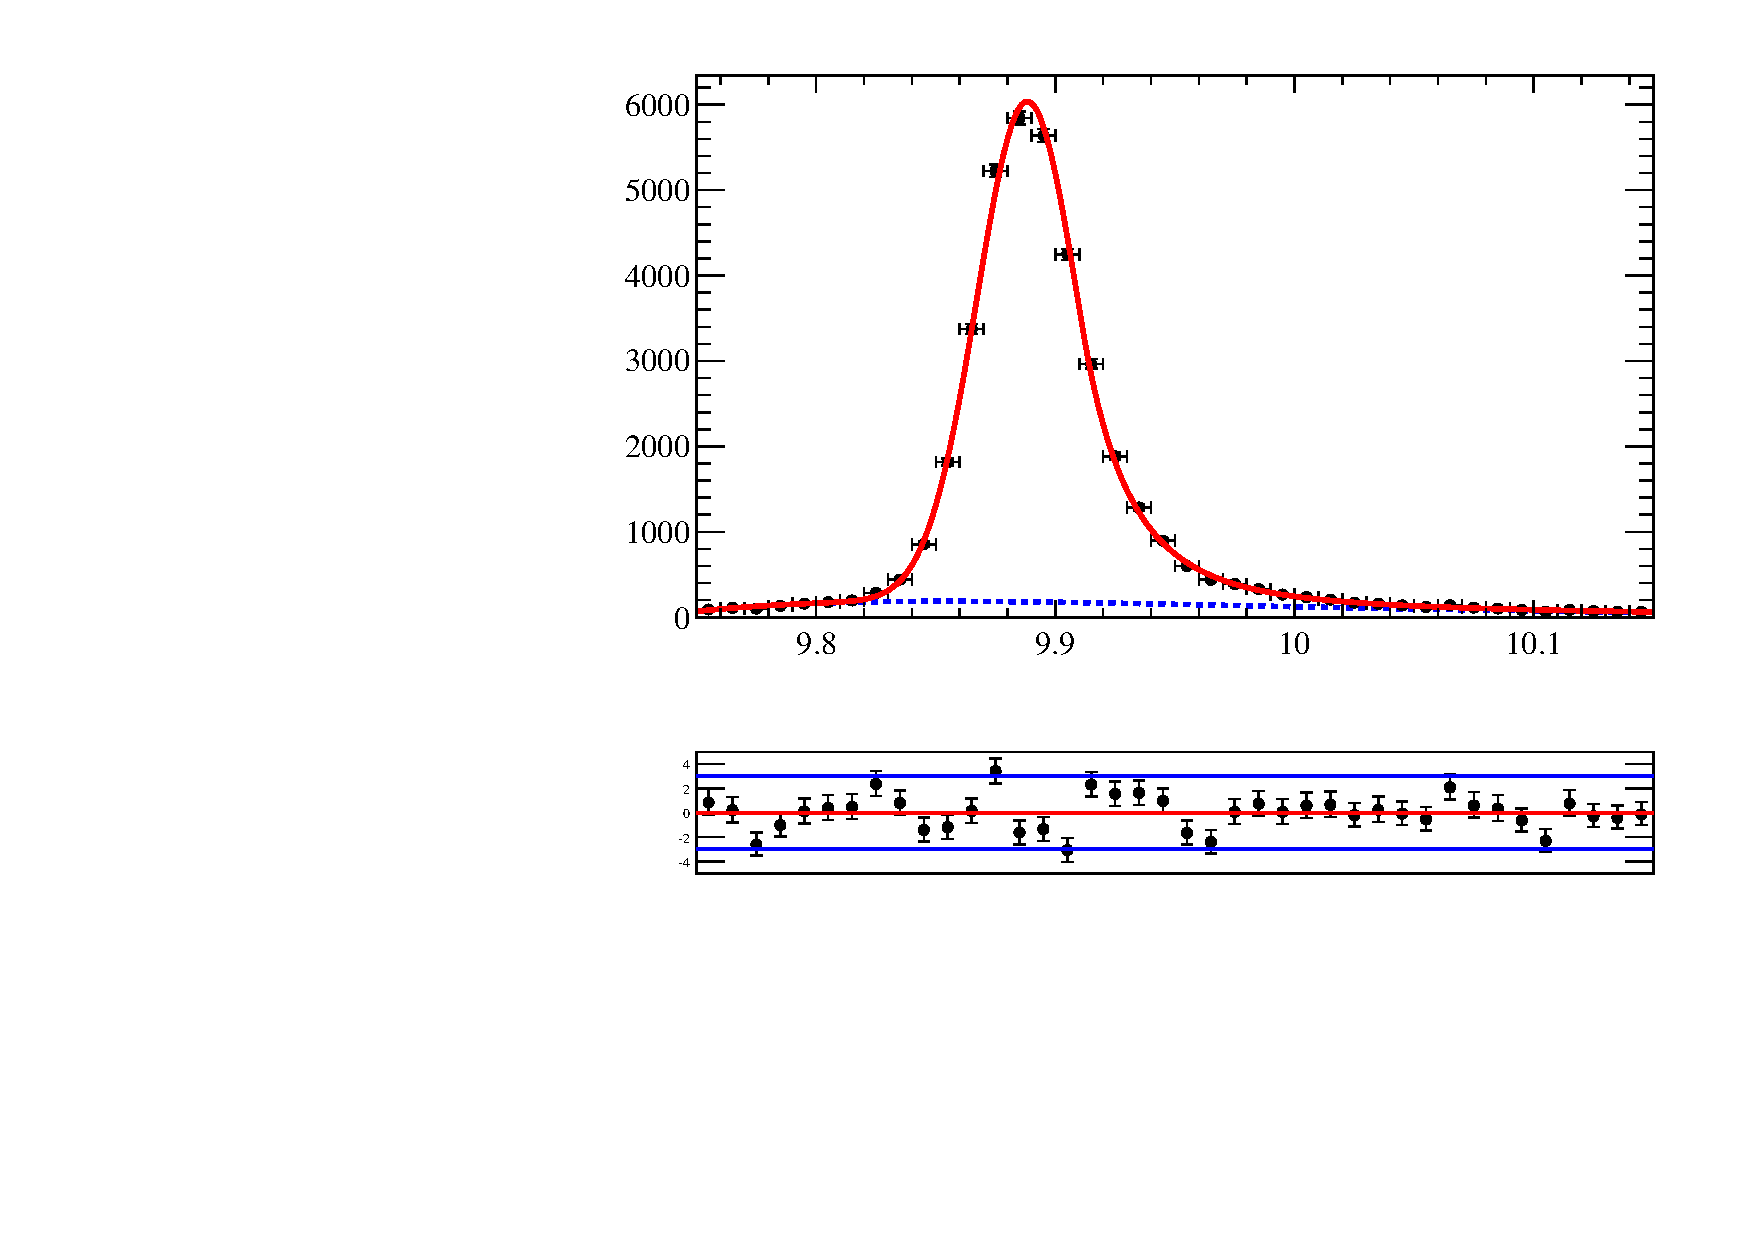
\includegraphics[width=75mm, height=60mm]{mc-fits-figs/cb11_6_40}
    }
    \put(42,114){\scriptsize $\chiboneOneP \to \Y1S \gamma$}
    \put(42,109){\scriptsize $6 < p_T^{\Y1S} < 40 \gevc$}
    \put(10,73){$m_{\mumu \gamma} - m_{\mumu} + m_{\Y1S}^{PDG} \left[\gevcc\right]$}
    \put(3,85){\scriptsize \begin{sideways}Candidates/(10\mevcc)\end{sideways}}    
    % \put(45,103){\scriptsize N = 34,330 $\pm$ 220}
    % \put(45,100){\scriptsize B = 5240 $\pm$ 140 (13.3 $\pm$ 0.4\%)}
    

    \put(75,60){
      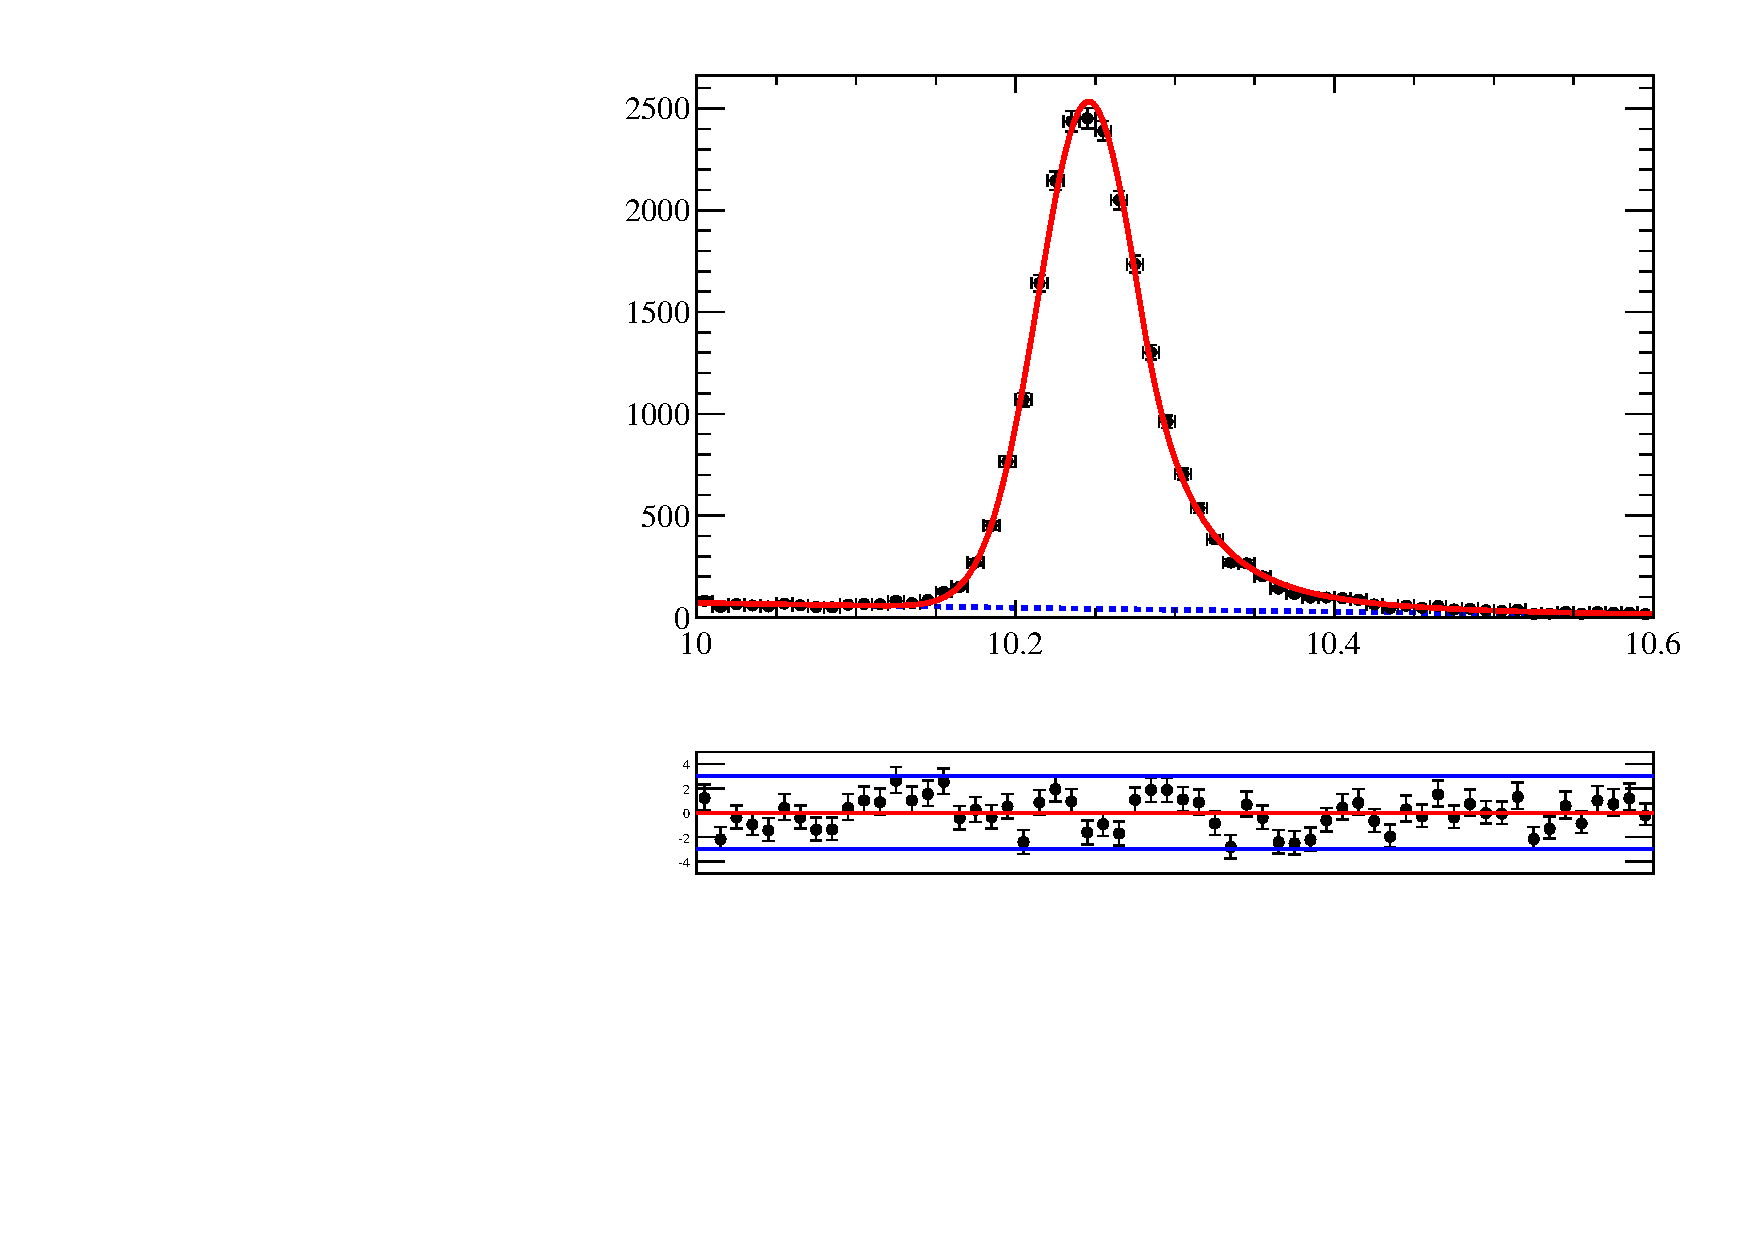
\includegraphics[width=75mm, height=60mm]{mc-fits-figs/cb12_6_40}
    }
    \put(117,114){\scriptsize $\chiboneTwoP \to \Y1S \gamma$}
    \put(117,109){\scriptsize $6 < p_T^{\Y1S} < 40 \gevc$}
    \put(85,73){$m_{\mumu \gamma} - m_{\mumu} + m_{\Y1S}^{PDG} \left[\gevcc\right]$}
    \put(78,85){\scriptsize \begin{sideways}Candidates/(10\mevcc)\end{sideways}}    
    % \put(120,103){\scriptsize N = 22,210 $\pm$ 170}
    % \put(120,100){\scriptsize B = 2290 $\pm$ 90 (9.3 $\pm$ 0.4\%)}
    

    \put(150,60){
      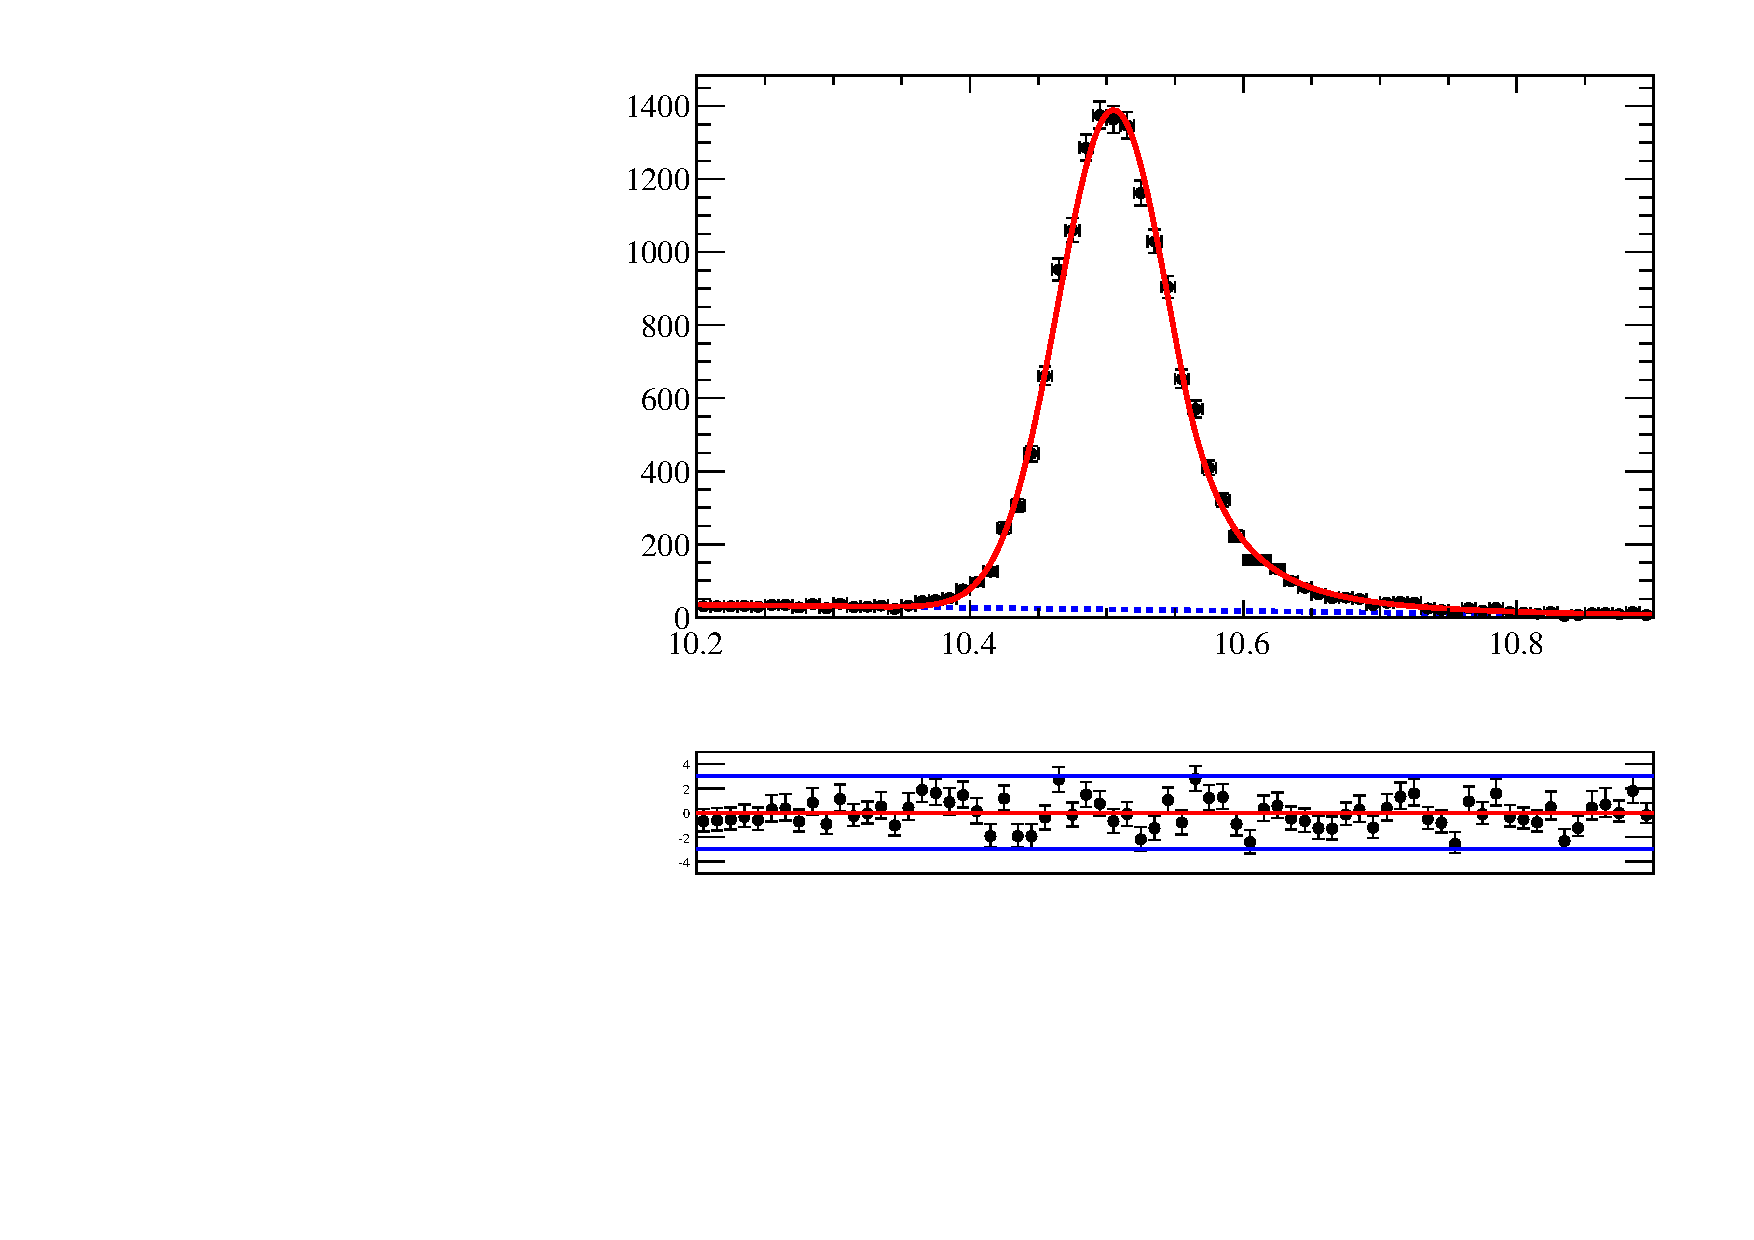
\includegraphics[width=75mm, height=60mm]{mc-fits-figs/cb13_6_40}
    }
    \put(192,114){\scriptsize $\chiboneThreeP \to \Y1S \gamma$}
    \put(192,109){\scriptsize $6 < p_T^{\Y1S} < 40 \gevc$}
    \put(160,73){$m_{\mumu \gamma} - m_{\mumu} + m_{\Y1S}^{PDG} \left[\gevcc\right]$}
    \put(153,85){\scriptsize \begin{sideways}Candidates/(10\mevcc)\end{sideways}}    
    % \put(195,103){\scriptsize N = 15,110 $\pm$ 130}
    % \put(195,100){\scriptsize B = 1360 $\pm$ 60 (8.26 $\pm$ 0.35\%)}
    

    \put(0,0){
      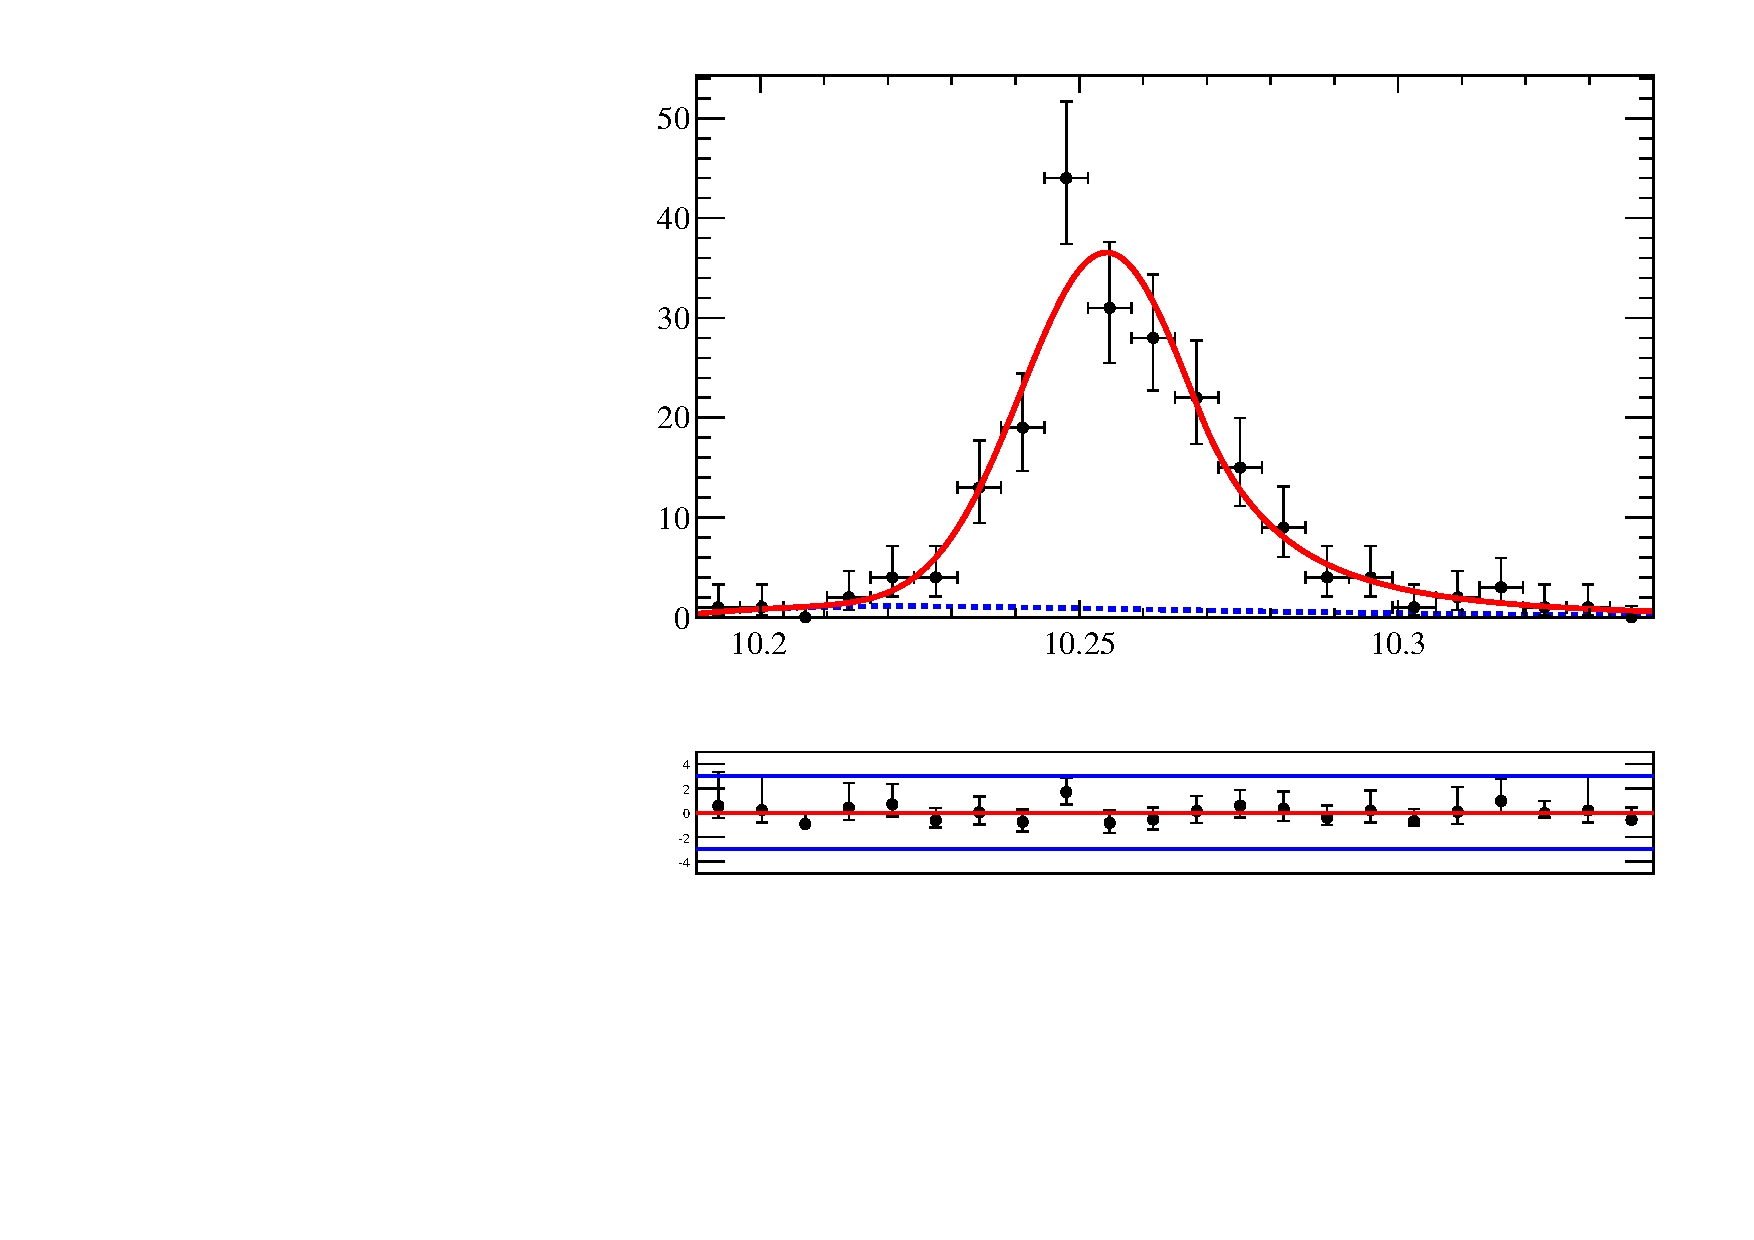
\includegraphics[width=75mm, height=60mm]{mc-fits-figs/cb12_18_40}
    }
    \put(42,54){\scriptsize $\chiboneTwoP \to \Y2S \gamma$}
    \put(42,49){\scriptsize $18 < p_T^{\Y2S} < 40 \gevc$}
    \put(10,13){$m_{\mumu \gamma} - m_{\mumu} + m_{\Y2S}^{PDG} \left[\gevcc\right]$}
    \put(3,25){\scriptsize \begin{sideways}Candidates/(10\mevcc)\end{sideways}}    
    % \put(45,43){\scriptsize N = 194 $\pm$ 21}
    % \put(45,40){\scriptsize B = 15 $\pm$ 17 (7 $\pm$ 8\%)}
    

    \put(75,0){
      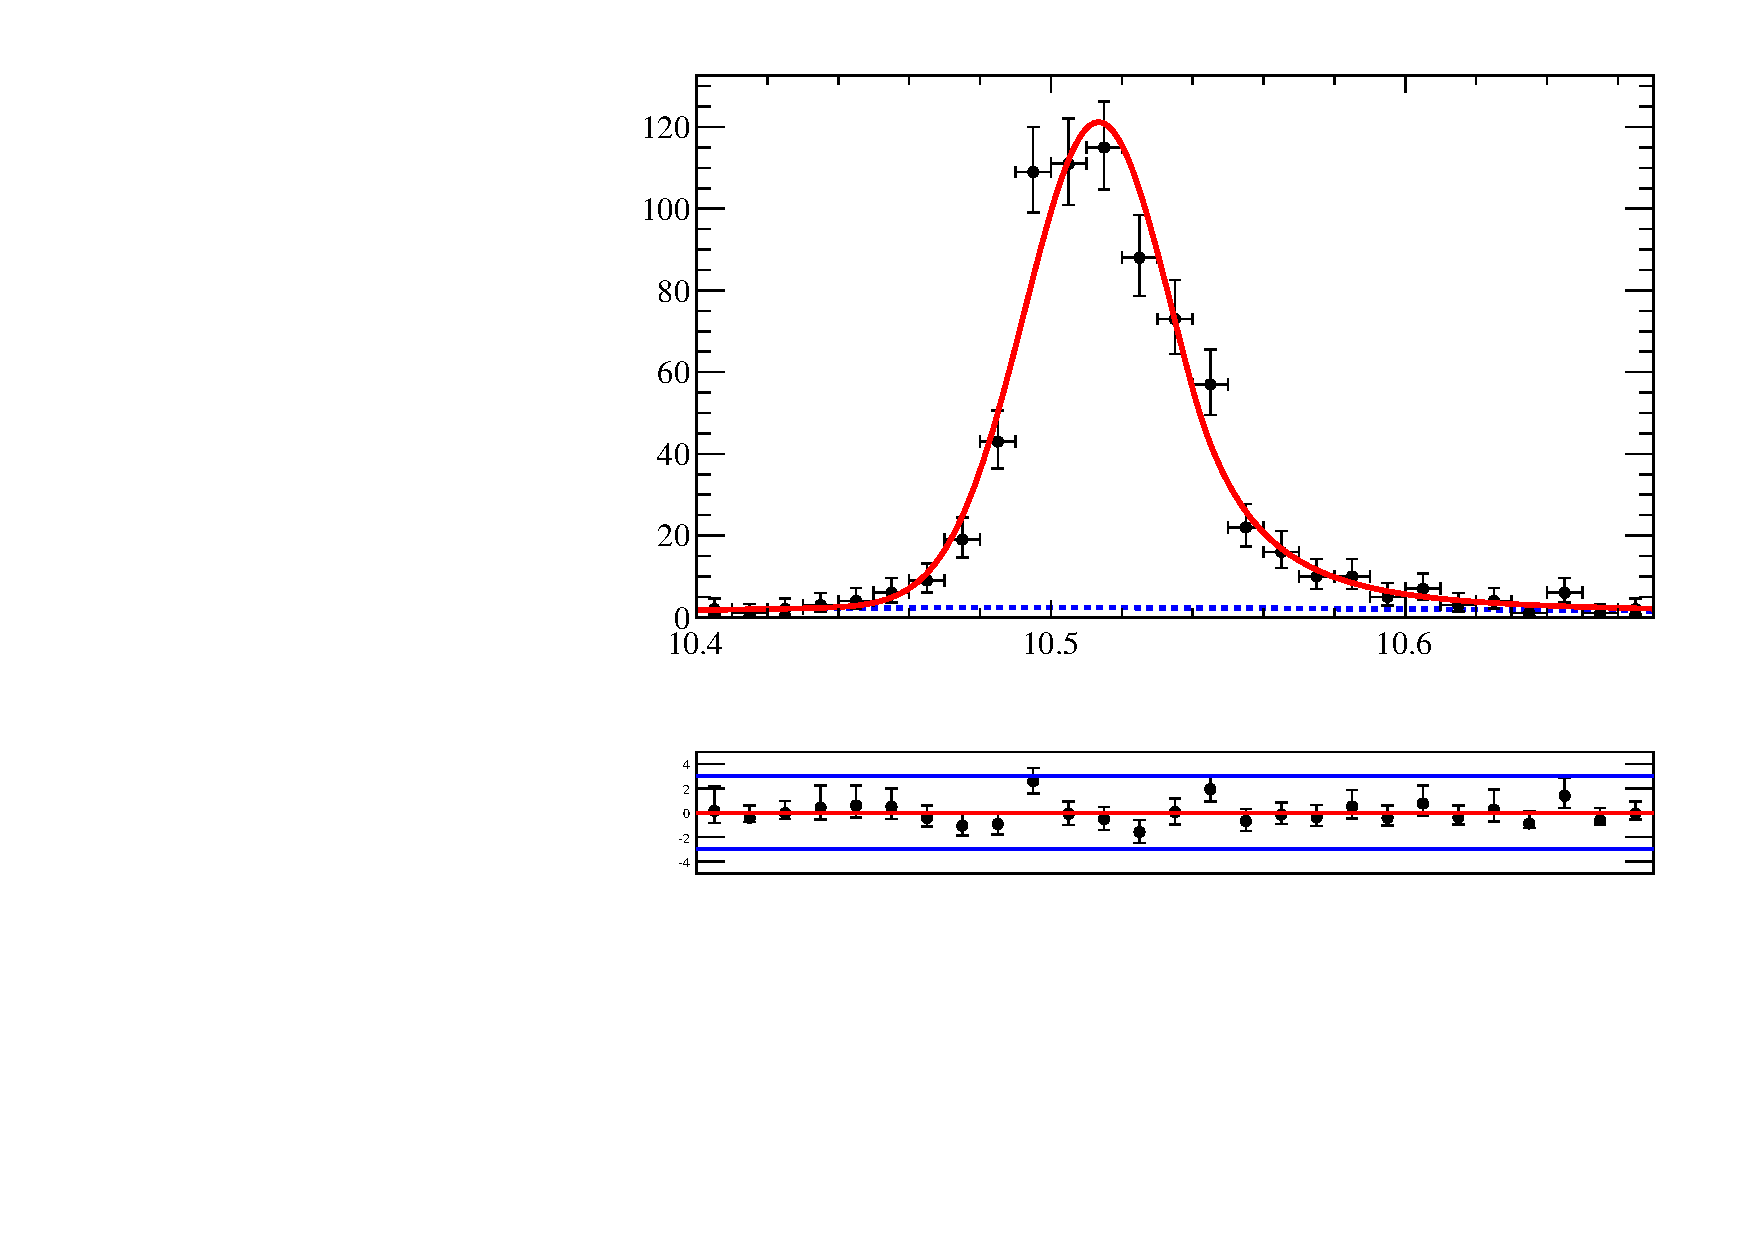
\includegraphics[width=75mm, height=60mm]{mc-fits-figs/cb13_18_40}
    }
    \put(117,54){\scriptsize $\chiboneThreeP \to \Y2S \gamma$}
    \put(117,49){\scriptsize $18 < p_T^{\Y2S} < 40 \gevc$}
    \put(85,13){$m_{\mumu \gamma} - m_{\mumu} + m_{\Y2S}^{PDG} \left[\gevcc\right]$}
    \put(78,25){\scriptsize \begin{sideways}Candidates/(10\mevcc)\end{sideways}}    
    % \put(120,43){\scriptsize N = 672 $\pm$ 32}
    % \put(120,40){\scriptsize B = 57 $\pm$ 21 (7.8 $\pm$ 2.9\%)}
    

    \put(150,0){
      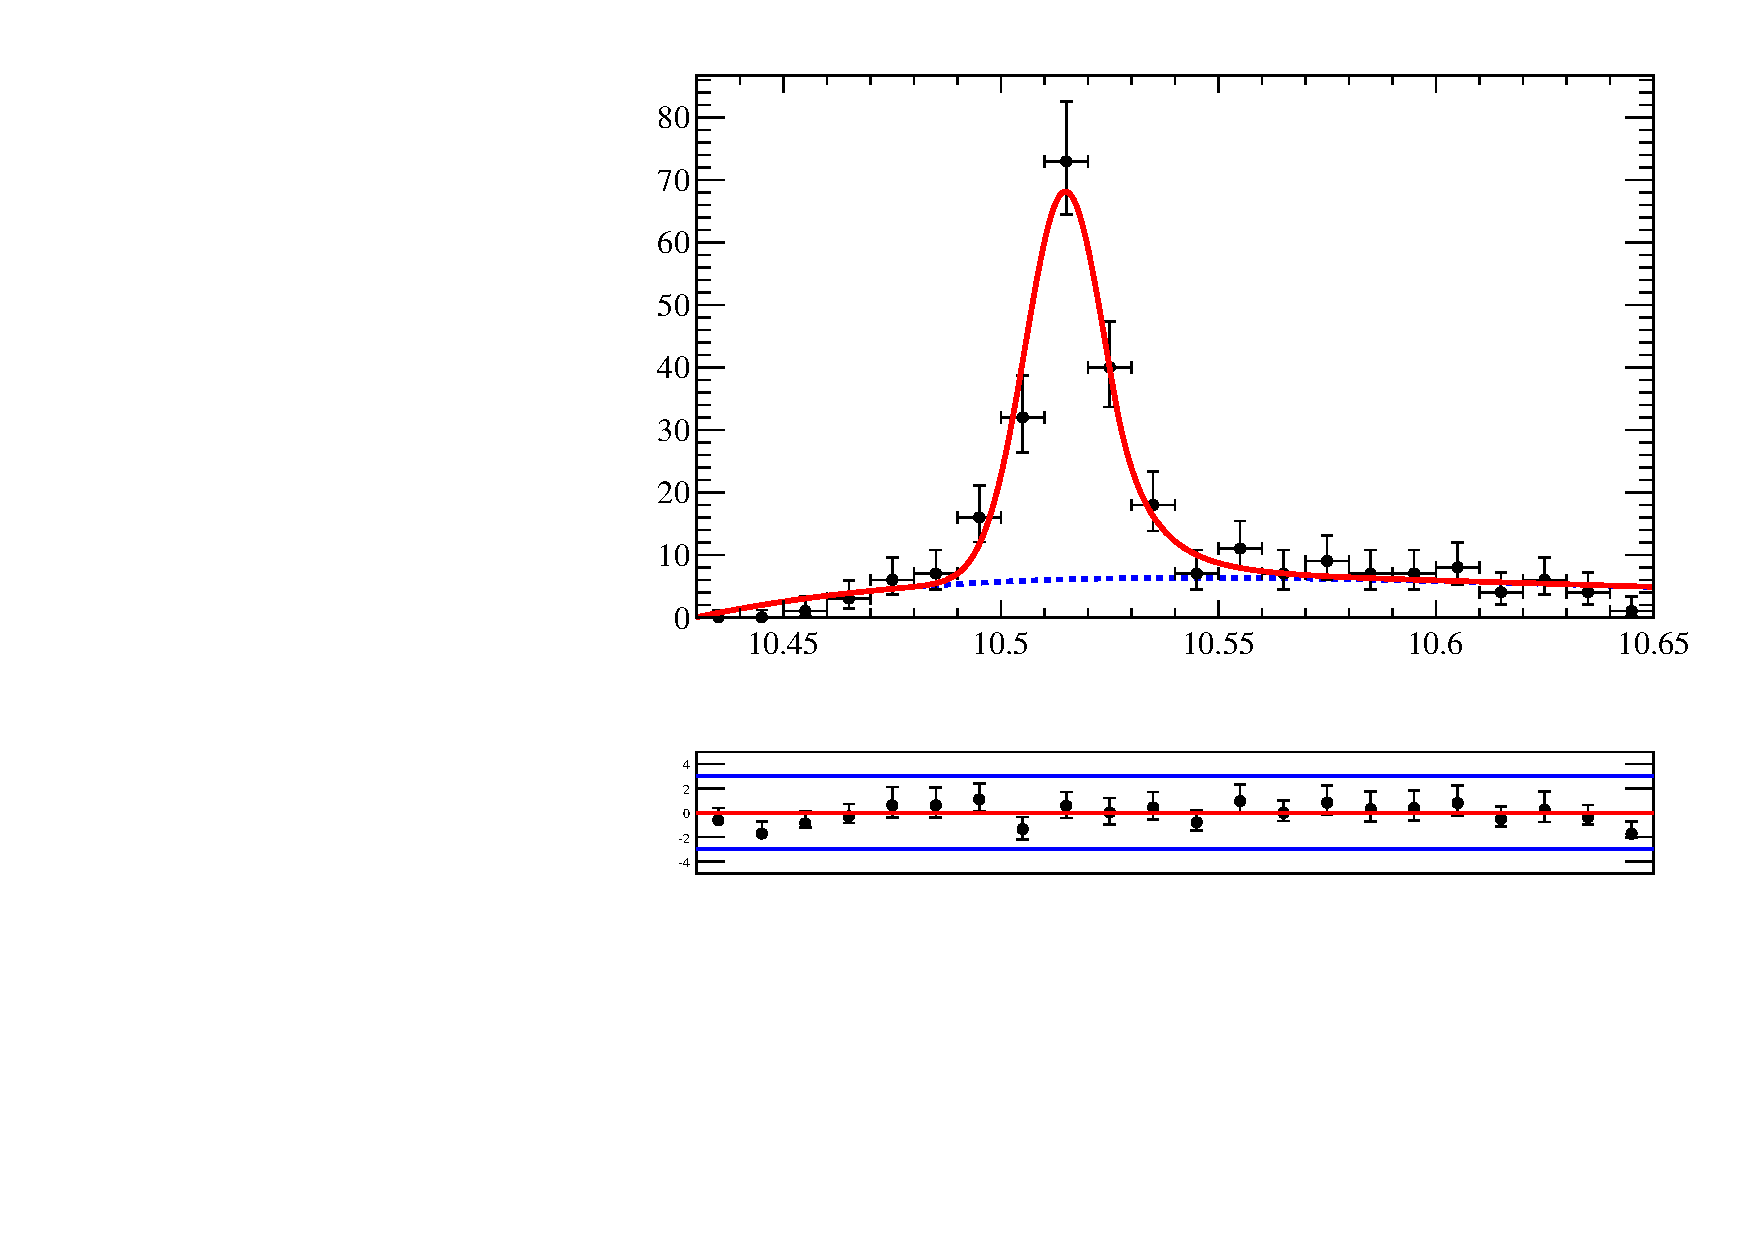
\includegraphics[width=75mm, height=60mm]{mc-fits-figs/cb13_27_40}
    }
    \put(192,54){\scriptsize $\chiboneThreeP \to \Y3S \gamma$}
    \put(192,49){\scriptsize $27 < p_T^{\Y3S} < 40 \gevc$}
    \put(160,13){$m_{\mumu \gamma} - m_{\mumu} + m_{\Y3S}^{PDG} \left[\gevcc\right]$}
    \put(153,25){\scriptsize \begin{sideways}Candidates/(10\mevcc)\end{sideways}}    
    % \put(195,43){\scriptsize N = 154 $\pm$ 17}
    % \put(195,40){\scriptsize B = 113 $\pm$ 16 (42 $\pm$ 7\%)}
    

     % \graphpaper[5](0,0)(225, 120)        
  \end{picture}
 }

\end{frame}